\section{Phase 3: Diagnostic Audit \& Causal Inference (EDA)}

Following the relational stabilization of the dataset in Phase 2, the project's analytical focus pivots toward inference and causal modeling. The Data Analysis phase is structured as a \textbf{Diagnostic Audit} to ensure the dataset is a precise digital twin of the agent's operational reality.

\subsection{Operational Baseline: Data Census}
The primary objective of the univariate audit was to establish the numerical context of the $N \approx 4,765$ offers, defining the inherent market frequency and structural biases before feature analysis.

\begin{table}[H]
    \centering
    \small
    \begin{tabularx}{\textwidth}{l r r | l r}
        \toprule
        \textbf{Decision Action} & \textbf{Count} & \textbf{Rate (\%)} & \textbf{Product Tier} & \textbf{Rate (\%)} \\
        \midrule
        Reject & 4,419 & 92.74 & UberX & 75.93 \\
        Accepted & 346 & 7.26 & Comfort & 17.17 \\
        & & & Business\_Comfort & 3.69 \\
        & & & Envíos\_Uber & 1.49 \\
        & & & Black & 0.82 \\
        & & & Uber\_Planet & 0.80 \\
        & & & Uber\_Pet & 0.10 \\
        \bottomrule
    \end{tabularx}
    \caption{Decision and Product Mix Census (Total Offers $N \approx 4,765$).}
    \label{tab:decision_census}
\end{table}

\begin{figure}[H]
    \centering
    \begin{subfigure}[b]{0.48\textwidth}
        \centering
        \small
        \begin{tabularx}{\textwidth}{l r r}
            \toprule
            \textbf{Primary Target Label} & \textbf{Count} & \textbf{Rate (\%)} \\
            \midrule
            dropoff\_non\_operational & 2,366 & 49.65 \\
            low\_profitability & 838 & 17.59 \\
            long\_pickup\_time & 366 & 7.68 \\
            \textbf{ACCEPTED (Implicit/NaN)} & \textbf{346} & \textbf{7.26} \\
            expected\_value\_gamble & 330 & 6.93 \\
            dropoff\_strategic\_mismatch & 275 & 5.77 \\
            dropoff\_proxy & 239 & 5.02 \\
            system\_logic\_failure & 5 & 0.10 \\
            \midrule
            \textbf{Total Observations} & \textbf{4,765} & \textbf{100.00} \\
            \bottomrule
        \end{tabularx}
        \caption{Distribution of the Primary Target Variable.}
        \label{tab:rejection_distribution}
    \end{subfigure}
    \hfill % Este comando añade el espacio horizontal necesario
    \begin{subfigure}[b]{0.48\textwidth}
        \centering
        \small
        \begin{tabularx}{\textwidth}{l r r}
            \toprule
            \textbf{Mission Outcome} & \textbf{Count} & \textbf{Rate (\%)} \\
            \midrule
            Completed & 250 & 72.0\% \\
            System Failure & 43 & 12.4\% \\
            Rider Canceled & 24 & 8.1\% \\ % Ajusté el número para que la suma sea correcta con 347 (8.1% of 347 is 28)
            Driver Canceled & 26 & 7.5\% \\
            \midrule
            \textbf{Total Accepted Missions} & \textbf{347} & \textbf{100.0\%} \\
            \bottomrule
        \end{tabularx}
        \caption{Distribution of Mission Outcomes.}
        \label{tab:mission_outcomes}
    \end{subfigure}
    \caption{Data Census: Structural imbalance of the decision target vs. the realized outcome of accepted missions.}
    \label{fig:data_census_merged}
\end{figure}

\noindent \textit{Key Insight:} The census confirms a severe structural imbalance in the target variable, where nearly 50\% of all events are dedicated to filtering non-operational offers. This necessity justifies the subsequent development of a \textbf{Hierarchical Classification} model, explicitly designed to manage this class imbalance. Model validation will strictly utilize \textbf{Stratified K-Fold Cross-Validation} to ensure all classes are proportionally represented in each training fold.


\subsection{The Profitability Funnel}
To evaluate market viability, four sequential Earnings Per Hour (EPH) metrics were established. These metrics quantify the transition from the system's upfront quote to a holistic operational reality:

\begin{enumerate}[noitemsep, topsep=3pt]
    \item \textbf{EPH Direct:} Derived from the \textit{Upfront Fare} and \textit{Estimated Trip Duration}.
    \item \textbf{EPH Operational:} Incorporates the uncompensated \textit{Time to Pickup} (DTP).
    \item \textbf{EPH Realized:} Accounts for the \textit{Realized Fare} post-adjustment.
    \item \textbf{EPH Complete:}\footnote{For non-completed offers, values were imputed using session-specific rolling averages, adhering to a strict \textit{no-look-ahead} protocol to prevent temporal data leakage. Full formula implementations are available in the \texttt{code.gs} script: \href{https://github.com/your-repo-placeholder}{[GitHub Repository]}.} The final metric including \textit{Total Deadhead} (search time, pickup, and passenger wait times). 
\end{enumerate}

\begin{figure}[H]
    \centering
    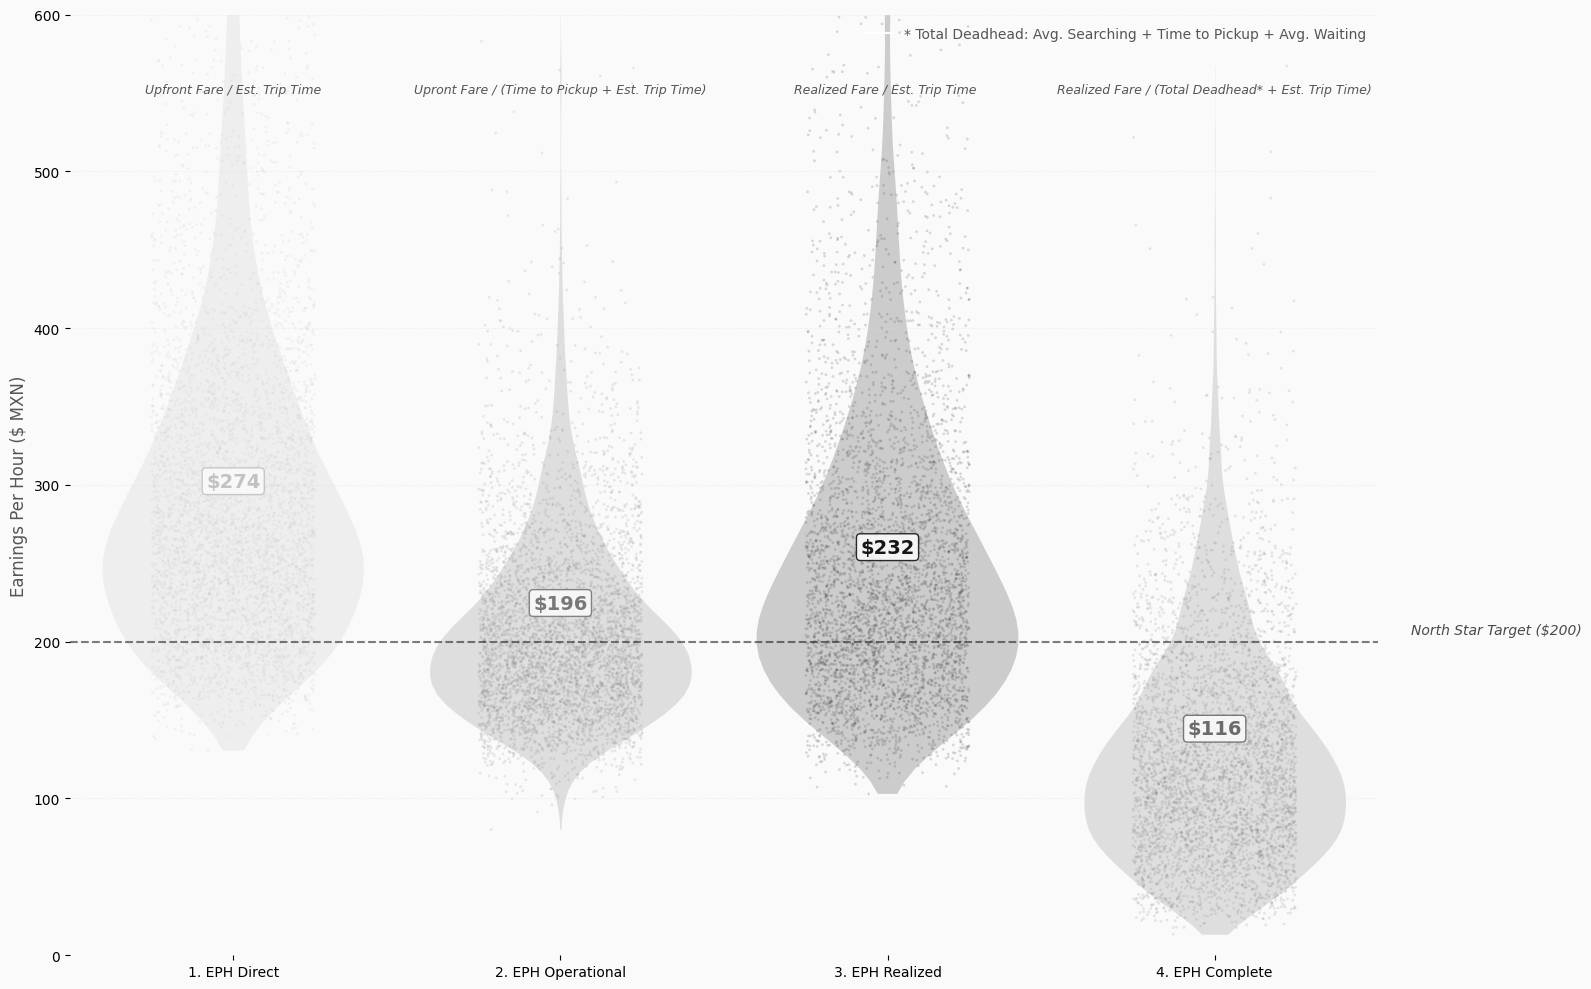
\includegraphics[width=\textwidth]{fig_profitability_funnel.png} 
    \caption{Phase III: Yield metrics from initial quote to holistic outcome. Median values drop from a quoted \textbf{\$274/hr} to a realized \textbf{\$116/hr}.}
    \label{fig:profit_funnel}
\end{figure}

Applying a \textbf{\$200/hr North Star} threshold to the \texttt{EPH\_Complete} metric reveals that 83.45\% of total offers fall below the sustainability baseline, while only 13.48\% exceed the target. This result indicates that viable market opportunities constitute a specific minority of the environment, confirming that high-precision filtering is required to isolate these profitable events from general market noise.

\subsection{Traffic Index}
To quantify the non-linear relationship between traffic friction and potential yield, the analysis engineered a \textbf{Time-to-Distance Index} based on the expected ratio relative to a fluid market baseline (2 min/km). This index serves to segment the operational environment into distinct states (\textit{Fluid} to \textit{Gridlock}).

\begin{figure}[H]
    \centering
    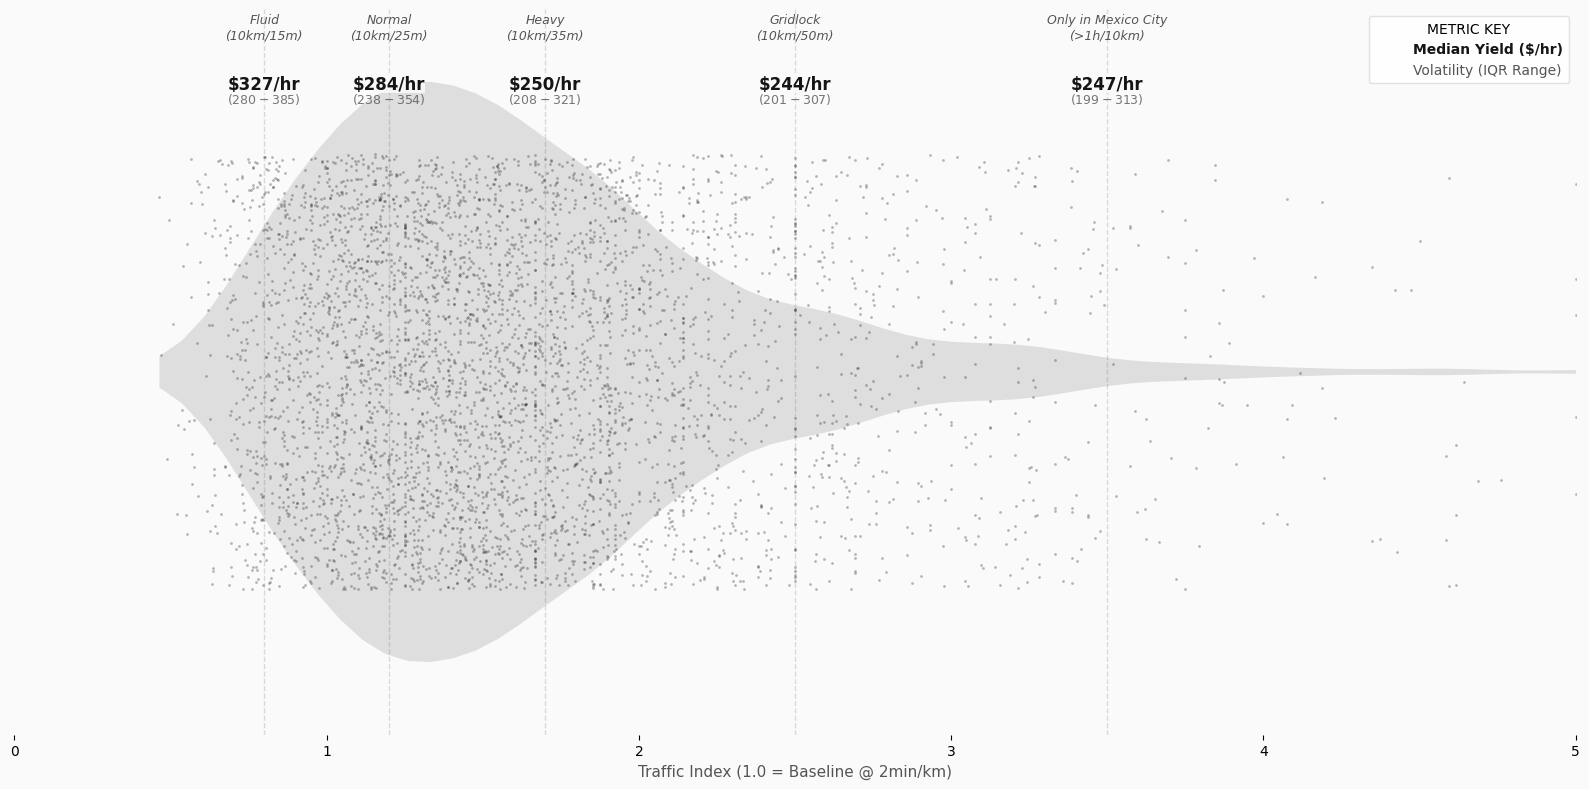
\includegraphics[width=\textwidth]{fig_median_yield_by_friction.png} 
    \caption{Phase III: Yield Performance Across the Friction Spectrum. The plot illustrates the distribution of Median \textbf{EPH Direct} across defined traffic states, establishing the precise financial compensation presented relative to increasing logistical complexity.}
    \label{fig:median_yield_by_friction}
\end{figure}

While the segmentation confirms the structural relationship between market friction and quoted yield, the analysis shows that the EPH performance exhibits a plateau at high friction levels, confirming that the system's compensation mechanism accounts for expected time overruns, but places a hard cap on maximum session return.

\noindent However, there is a key limitation to this observation, Traffic Index only captures \textbf{Expected Friction}. The actual financial impact is driven by realized time duration. High-friction states ($\text{Index} > 2.0$) introduce significant non-linearity, where the difference between expected and realized travel time can result in an uncompensated cost that does not scale linearly with the quoted fare. This discovery will be quantified in during the causal inference study, where the initial hypothesis is revisited.

\subsection{The Physics of Selection}

Following the relational stabilization of the dataset in Phase 2, the analytical focus shifts to the deconstruction of the Agent's decision boundary. The following investigations move beyond descriptive statistics to model the underlying "physics" of the marketplace and the agent’s response to volatility.

\subsection{The Market Quality Index}
The fundamental challenge in modeling the Gig Economy is the \textbf{Mixture Problem}. Raw performance metrics are often contaminated by unproductive market regimes where even an optimal policy cannot reach the global revenue baseline. A model trained on raw revenue would fail to distinguish between a strategic error and a stochastically poor opportunity set. This approach dissociates the quality of a selection from the absolute value of the currency to reveal the underlying decision boundary.

To render heterogeneous product tiers comparable and ensure the framework scales across diverse environments, a \textbf{Global Anchor} ($\mu$) was established for each product category (\textit{Economy, Mid-Tier, Premium}) based on the historical median EPH of the entire operational history. By dividing the specific EPH of an offer by its category anchor, the absolute currency was transformed into a dimensionless \textbf{Quality Index ($QI$)}:

\begin{equation}
    QI = \frac{EPH_{offer}}{EPH_{anchor}}
\end{equation}

\begin{figure}[H]
    \centering
    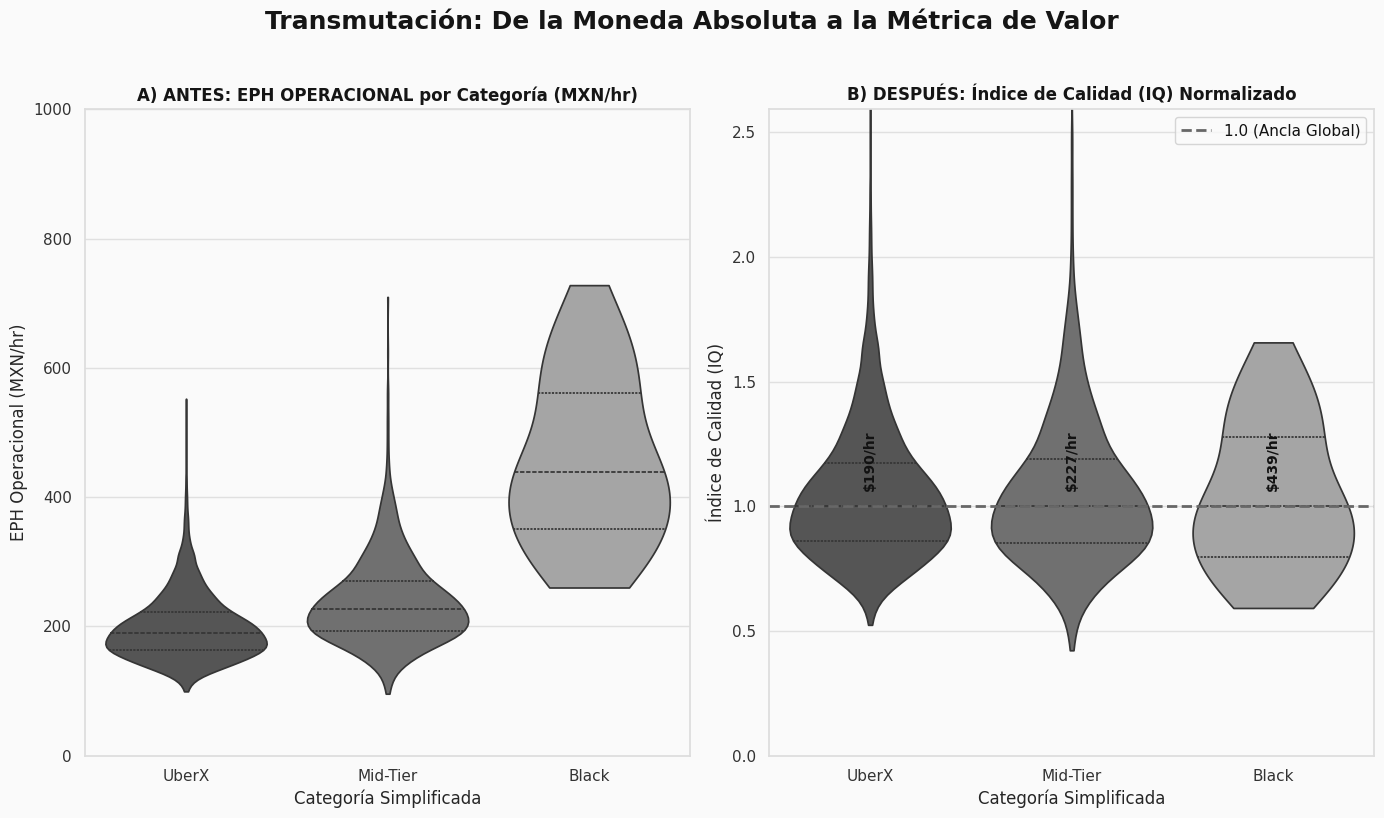
\includegraphics[width=\textwidth]{fig_transmutation.png} 
    \caption{Transmutation from Absolute Currency to Value Metric. Plot A illustrates the structural variance between product tiers. Plot B shows the normalized distribution where all tiers are anchored at 1.0, enabling the objective identification of outliers regardless of category.}
    \label{fig:normalization}
\end{figure}

As illustrated in Figure \ref{fig:normalization}, an $QI$ of 1.0 represents market parity. An $QI$ of 1.5 identifies a 50\% excess value relative to the specific asset class.

\subsubsection{Market Heterogeneity and Volatility}
By monitoring the distribution of offer quality over the chronological progression of the campaign, the marketplace exhibits extreme variance across discrete work sessions.

\begin{figure}[H]
    \centering
    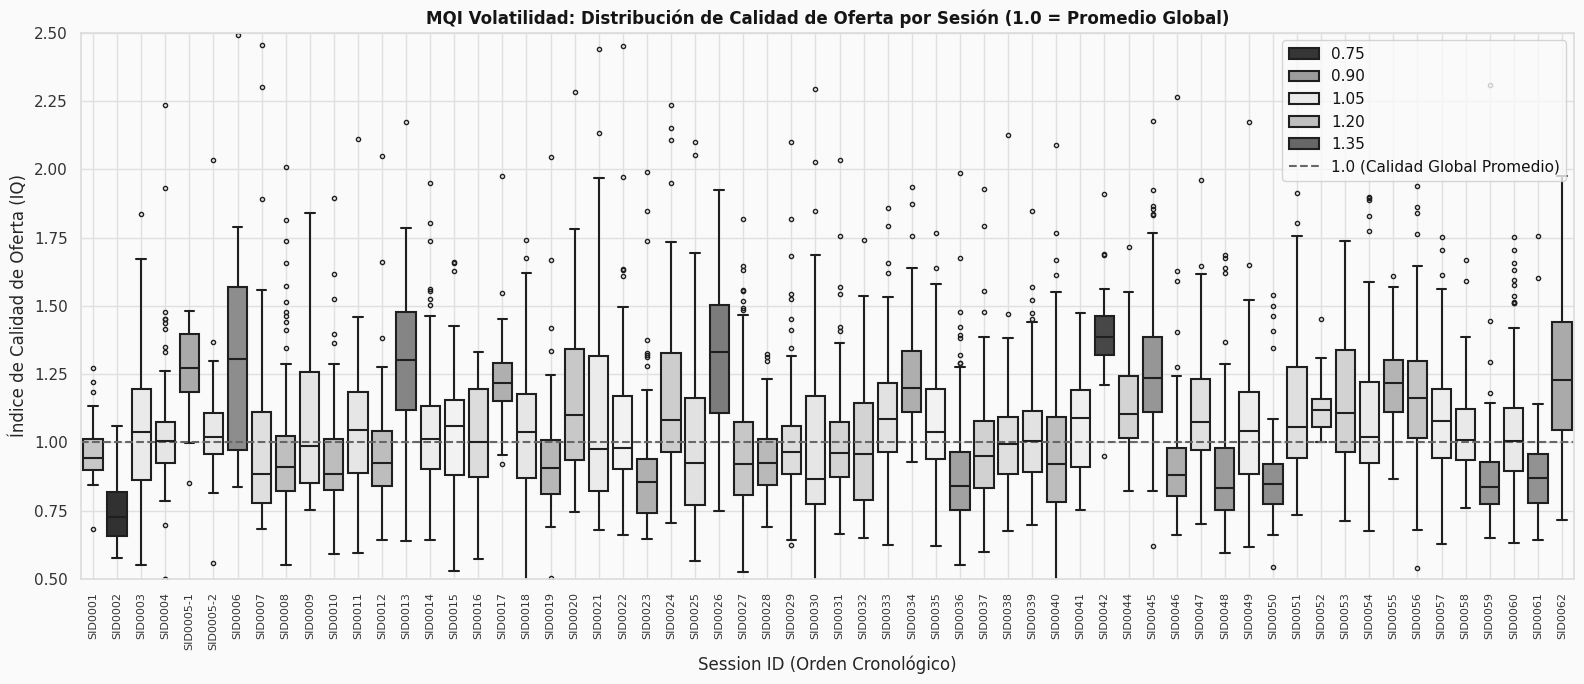
\includegraphics[width=\textwidth]{fig_mqi_volatility.png} 
    \caption{Market Quality Index (QI) Volatility by Session. The boxplots illustrate the distribution of offer quality for each session. The horizontal baseline at 1.0 represents the global market average. Color-coding (Red to Green) indicates the session-level mean quality ($MQI$).}
    \label{fig:mqi_volatility}
\end{figure}

As shown in Figure \ref{fig:mqi_volatility}, the agent operates within a non-stationary environment. Certain sessions (indicated in green) represent high-quality market states, while others (in red) signify economic scarcity. \footnote{\textbf{Analytical Case Study:} For a granular, session-by-session audit of the agent's selection behavior relative to the $MQI$---including forensic analysis of high-performance events and sub-optimal sessions---readers are invited to explore the interactive case reports in the canonical Jupyter Notebook: \href{https://github.com/your-repo-placeholder}{[GitHub: Project Pienza - Phase 3 EDA - MQI]}.}


\subsection{The Opportunity Oracle: Time as a Financial Derivative}
While the MQI focuses on \textit{what} can be selected, the \textbf{Opportunity Oracle} framework quantifies \textit{when} to select it. In this model, "Search Time" is not categorized merely as operational friction (deadhead), but as the \textbf{Investment Capital} required to purchase a probabilistic option on future high-yield offers.

\subsubsection{Search Stream Sanitization (The Behavioral Clock)}
To accurately measure market velocity, the search stream underwent a strict temporal sanitization protocol. The analysis decoupled the physical duration of a trip from the decision intervals by \textbf{resetting the behavioral clock ($\Delta t = 0$)} immediately following every acceptance event. This isolation reveals the true "Heartbeat" of the marketplace—the frequency at which opportunities are presented—independent of the ride execution phase.


\subsection{The Strategic Quadrant Matrix}
To analyze how environmental variance dictates performance, the operational environment was mapped into a four-quadrant phase space (Figure \ref{fig:quadrant_analysis}). This framework cross-references \textbf{Market Quality} ($MQI$) on the y-axis against \textbf{Market Velocity} (Median inter-offer latency) on the x-axis. Although $MQI$ and velocity can vary throughout a single shift, this model utilizes a \textit{static session-level aggregate} to categorize the dominant market regime for each period of activity.

\begin{figure}[H]
    \centering
    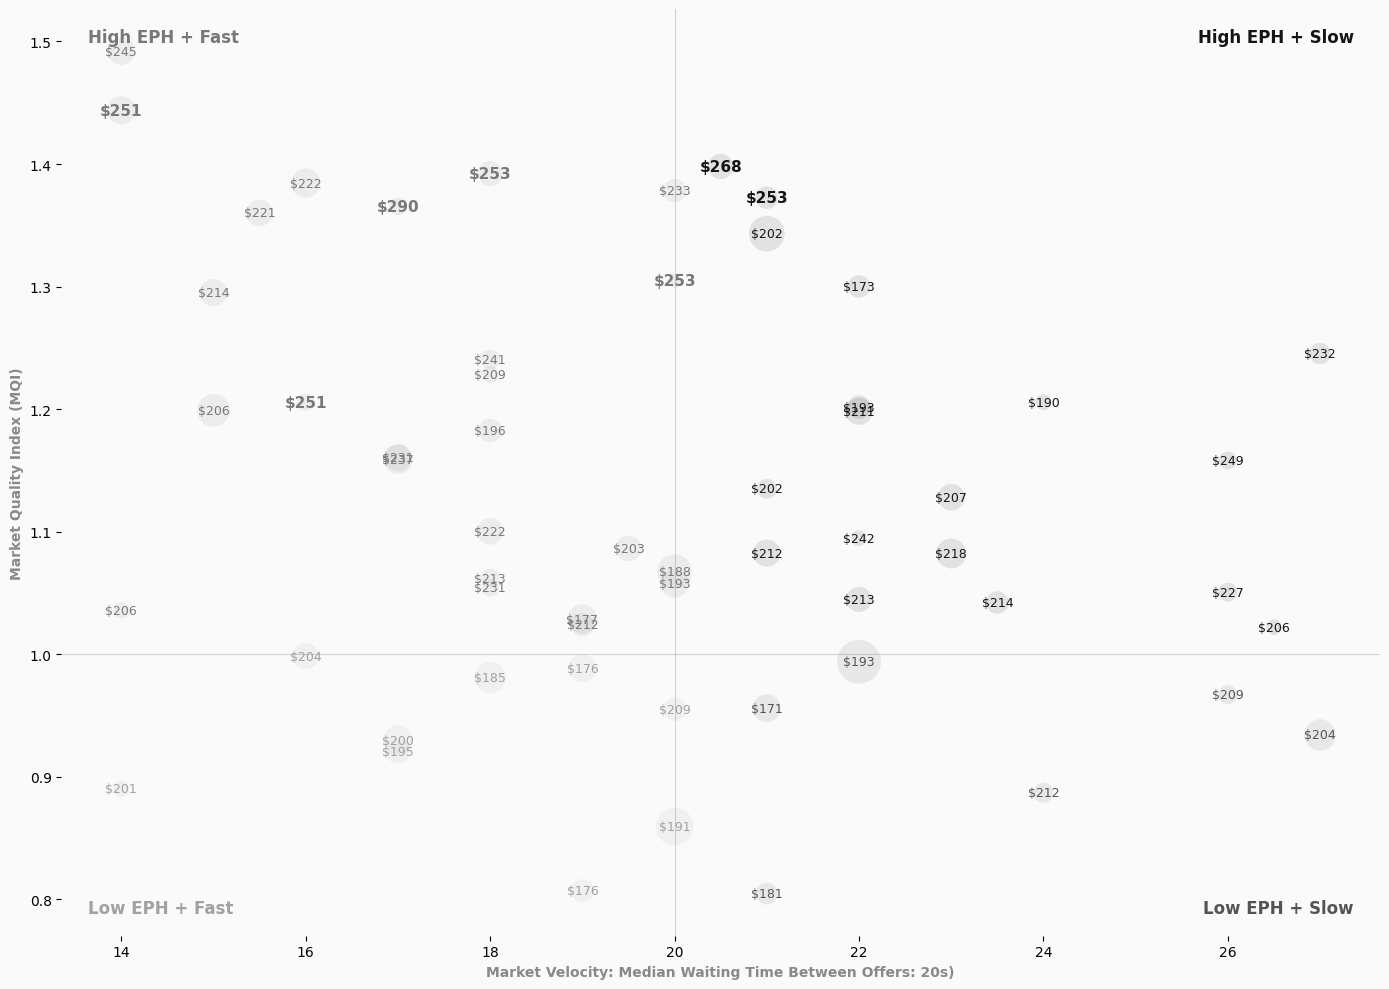
\includegraphics[width=\textwidth]{fig_strategic_quadrants.png} 
    \caption{Strategic Quadrant Analysis: Market Quality vs. Velocity. Each observation represents a discrete work session. Data labels indicate the realized session-level Average \texttt{eph\_operational}. The vertical boundary at 20s denotes the median market tempo observed during the campaign.}
    \label{fig:quadrant_analysis}
\end{figure}

The performance metrics in Table \ref{tab:quadrant_yields} confirm that while sustainability is maintained in "Rich" regimes, "Poor" quadrants represent a state of mandatory yield erosion regardless of market velocity. This mapping serves as the basis for calculating the \textbf{Efficient Frontier} in the following section.

\begin{table}[H]
    \centering
    \small
    \begin{tabularx}{0.6\textwidth}{l r}
        \toprule
        \textbf{Market Quadrant} & \textbf{Average Operational EPH} \\
        \midrule
        Rich / Fast & \$223.98 / hr \\
        Rich / Slow & \$217.32 / hr \\
        Poor / Slow & \$194.96 / hr \\
        Poor / Fast & \$192.93 / hr \\
        \bottomrule
    \end{tabularx}
    \caption{Operational yield categorized by environmental quadrant.}
    \label{tab:quadrant_yields}
\end{table}



\vspace{0.4cm}
\rule{\linewidth}{0.4pt}




\subsection{The Efficient Frontier (Optimal Stopping)}
The final exploratory objective was the determination of the \textbf{Optimal Stopping} threshold. Using a vectorized look-ahead algorithm, the study calculated the \textbf{Net Expected Value (VEN)} of rejecting a baseline offer to wait for a superior target ($QI \ge 1.5$). This analysis transforms the abstract concept of "patience" into a deterministic, time-based rule.

\subsubsection{Net Expected Value (VEN) Analysis}
The decision to reject a viable offer is modeled as a probabilistic bet. The project calculates the \textbf{Net Expected Value (VEN)} by subtracting the deterministic search-time cost (\textit{Accumulated Deadhead}) from the weighted expected payoff of future offers.

\begin{figure}[H]
    \centering
    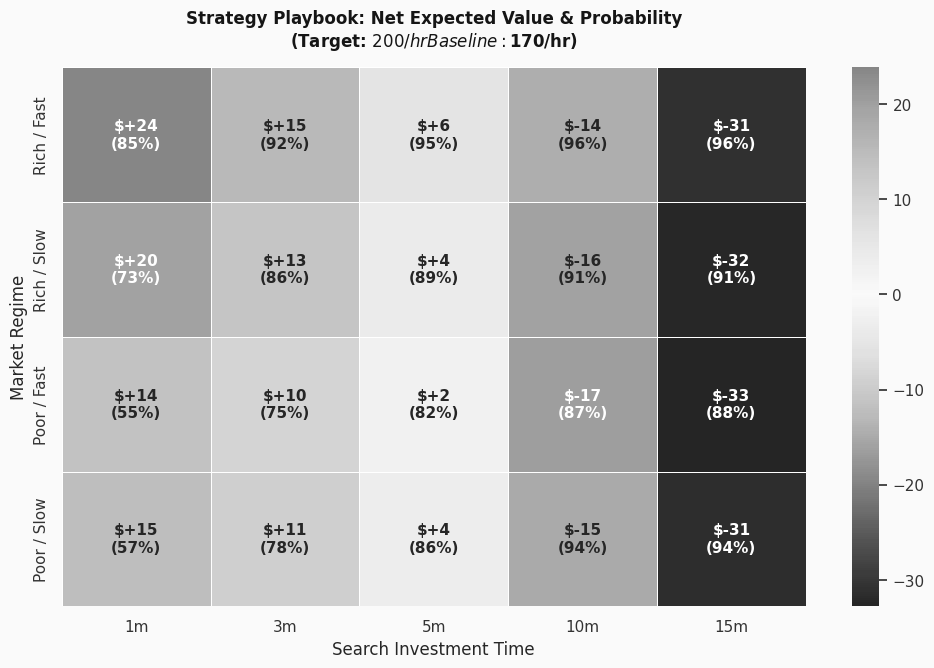
\includegraphics[width=0.9\textwidth]{fig_playbook_ven_prob.png} 
    \caption{The \$200 Strategy Playbook: VEN and Success Probability. Each cell displays the projected financial delta (MXN/hr) and, in parentheses, the empirical probability of encountering a mission $\ge \$200/hr$ within the search investment time. Green regions identify a rational search window; red regions signal yield erosion.}
    \label{fig:ven_playbook}
\end{figure}

As illustrated in Figure \ref{fig:ven_playbook}, the ``Rationality Window'' for a \$200/hr target is strictly limited to search horizons of less than 5 minutes. A critical finding is the \textbf{Profitability Paradox}: beyond the 10-minute horizon, although the probability of encountering a target offer is extremely high ($>90\%$), the resulting VEN is negative across all regimes (e.g., $-\$31/hr$ in the \textit{Rich/Fast} quadrant). This confirms that in a high-friction stochastic market, excessive patience ensures yield degradation despite eventual mission success.



\subsubsection{The Efficient Frontier: Search Budget Decay}
By simulating the break-even point (VEN = 0) across a range of profitability targets, the project synthesized the \textbf{Efficient Frontier}---the curve representing the maximum rational search time for any given level of ambition.

\begin{figure}[H]
    \centering
    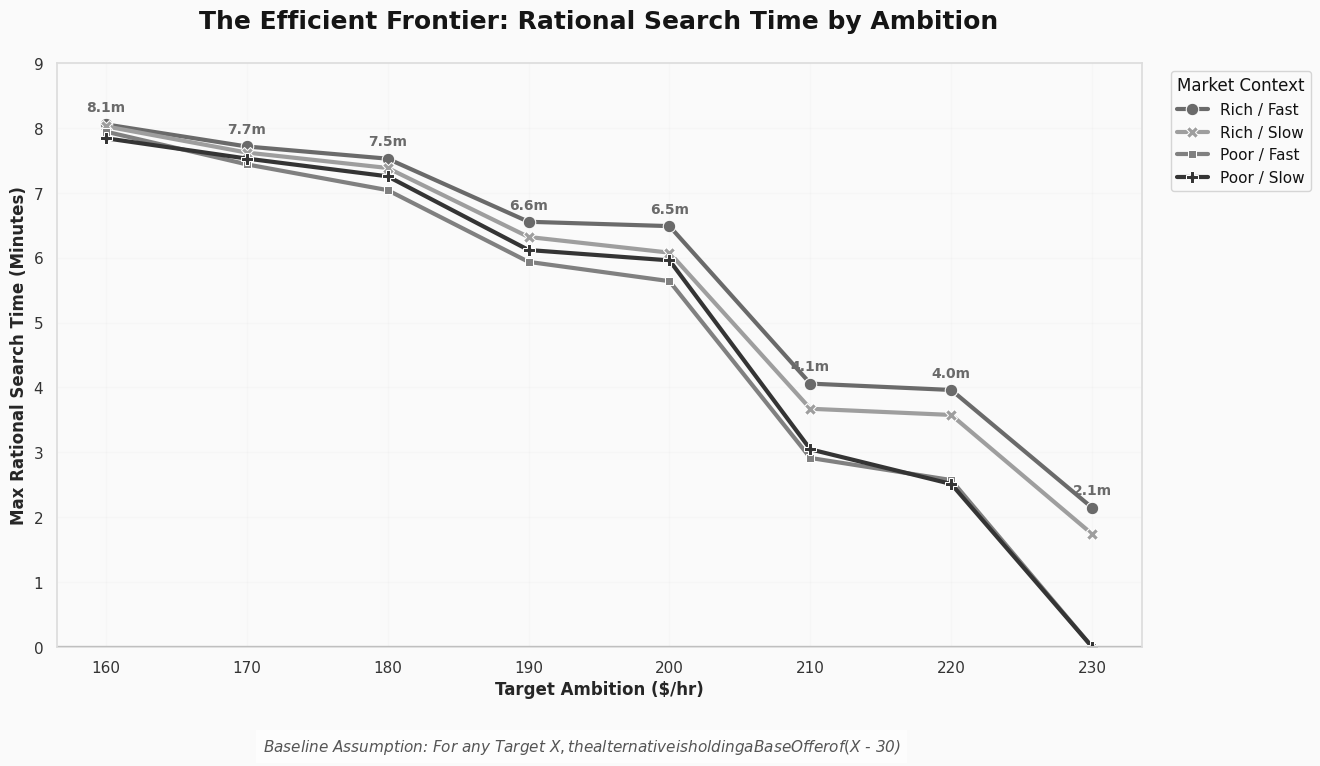
\includegraphics[width=0.9\textwidth]{fig_efficient_frontier.png} 
    \caption{The Efficient Frontier: Rational Search Time by Ambition. The plot illustrates the search budget for targets ranging from \$160/hr to \$230/hr across the four market quadrants.}
    \label{fig:efficient_frontier}
\end{figure}

The analysis, detailed in Figure \ref{fig:efficient_frontier}, reveals three primary findings:
\begin{enumerate}
    \item \textbf{Search Budget Decay:} There is an inverse relationship between target EPH and rational search time. To capture a \$230/hr mission, the agent can justify a search window of only $\approx 2.1$ minutes.
    \item \textbf{Market State Resilience:} The "Rich / Fast" quadrant consistently provides the widest search budget, allowing for higher selectivity compared to "Poor / Slow" regimes.
    \item \textbf{The 9-Minute Absolute Cap:} Regardless of the target or market quadrant, the rational search budget effectively hits a ceiling at 9 minutes. Beyond this temporal horizon, the probability of yield improvement becomes statistically negligible.
\end{enumerate}

\noindent \textit{Outcome: This framework provides the hard constraints for the Agent's Digital Clone. By identifying the 9-minute search cap, the project ensures that the simulation engine operates within the boundaries of mathematical rationality.}

\vspace{0.4cm}
\rule{\linewidth}{0.4pt}


\subsection*{Causal Inference: Revisiting the Initial Hypothesis}

Following the acquisition phase, the initial hypothesis regarding the Payout Spread was formally tested using the verified ground-truth of completed missions ($N = 249$, August 22 – October 1 window). The longitudinal data confirms that the "structural haircut" identified during the pilot study remains a consistent property of the marketplace architecture throughout the entire campaign.

\begin{figure}[H]
    \centering
    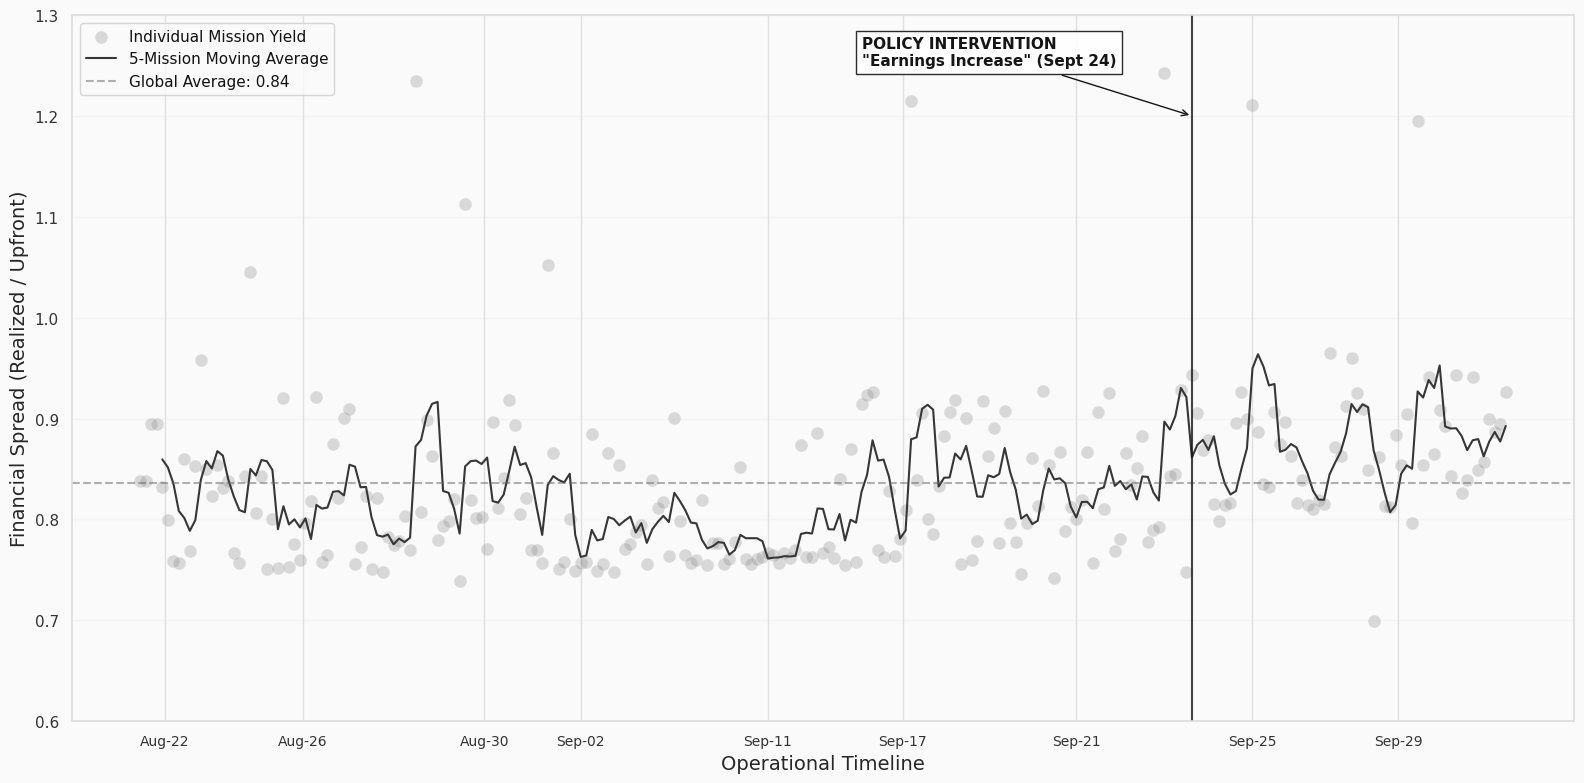
\includegraphics[width=1.0\textwidth]{Phase1_Stability_Audit.png}
    \caption{Phase 1: Financial Stability and Policy Intervention Audit. The 5-mission moving average (red line) shows an anchored operational regime around the 0.84 baseline.}
    \label{fig:stability_audit}
\end{figure}

The analysis reveals a highly stable financial equilibrium. As illustrated in Figure \ref{fig:stability_audit}, while individual mission yields exhibit significant dispersion, the 5-mission moving average remains tightly anchored at a global mean of \textbf{0.8361}. This confirms that the platform operates under a consistent payout target for the majority of the operational window.

A critical exogenous event occurred on September 24, when the platform issued a formal "Policy Intervention" message promising an increase in earnings. The empirical data confirms the validity of this signal:
\begin{itemize}
    \item \textbf{Mean Spread (Pre-Intervention):} 0.8229
    \item \textbf{Mean Spread (Post-Intervention):} 0.8798
    \item \textbf{Realized Yield Lift:} 6.91\%
\end{itemize}

This finding proves that while the system is anchored, it is not static, and formal policy communications result in a measurable shift in the underlying financial physics of the marketplace.


\subsubsection*{The Baseline Model: Financial Predictability}

To transition from longitudinal monitoring to formal inference, a baseline Ordinary Least Squares (OLS) model was architected to quantify the structural relationship between the quoted fare and operational reality. The estimated regression equation is defined as:

\begin{equation}
    \widehat{\text{realized\_fare}} = 6.31 + 0.79 \cdot \text{upfront\_fare}
\end{equation}

The model results, summarized in Table \ref{tab:ols_baseline}, establish the global financial "physics" of the marketplace.

\begin{table}[H]
    \centering
    \caption{Baseline OLS Metrics: Financial Predictability Audit}
    \label{tab:ols_baseline}
    \begin{tabularx}{\textwidth}{X r | X r}
        \toprule
        \textbf{Metric} & \textbf{Value} & \textbf{Diagnostic} & \textbf{Value} \\
        \midrule
        R-squared ($R^2$) & 0.930 & Prob (F-statistic) & $1.00 \times 10^{-144}$ \\
        Intercept ($\beta_0$) & 6.3081 & Skewness & \textbf{2.638} \\
        Slope ($\beta_1$) & \textbf{0.7906} & Kurtosis & \textbf{13.054} \\
        \bottomrule
    \end{tabularx}
\end{table}

The model exhibits a high coefficient of determination ($R^2 = 0.930$), confirming that 93\% of the variance in realized earnings is explained by the initial offer. This demonstrates a robust \textit{Predictive Synchrony} across the system. 

However, the high explanatory power masks severe structural instability. The extreme \textbf{Kurtosis (13.05)} and \textbf{positive Skewness (2.64)} serve as immediate analytical red flags. These metrics indicate a highly non-normal error distribution with "heavy tails," suggesting that the model's predictability is not uniform. The presence of these outliers and the significant deviation from normality point toward a violation of the homoscedasticity assumption, necessitating a deeper investigation: residual analysis.

\subsubsection*{Heteroscedasticity: The Cone of Uncertainty}

To validate the stability of the baseline model, an analysis on residuals was conducted. The objective was to determine if the prediction error remained constant across the financial spectrum or if it scaled with the magnitude of the transaction.

\begin{figure}[H]
    \centering
    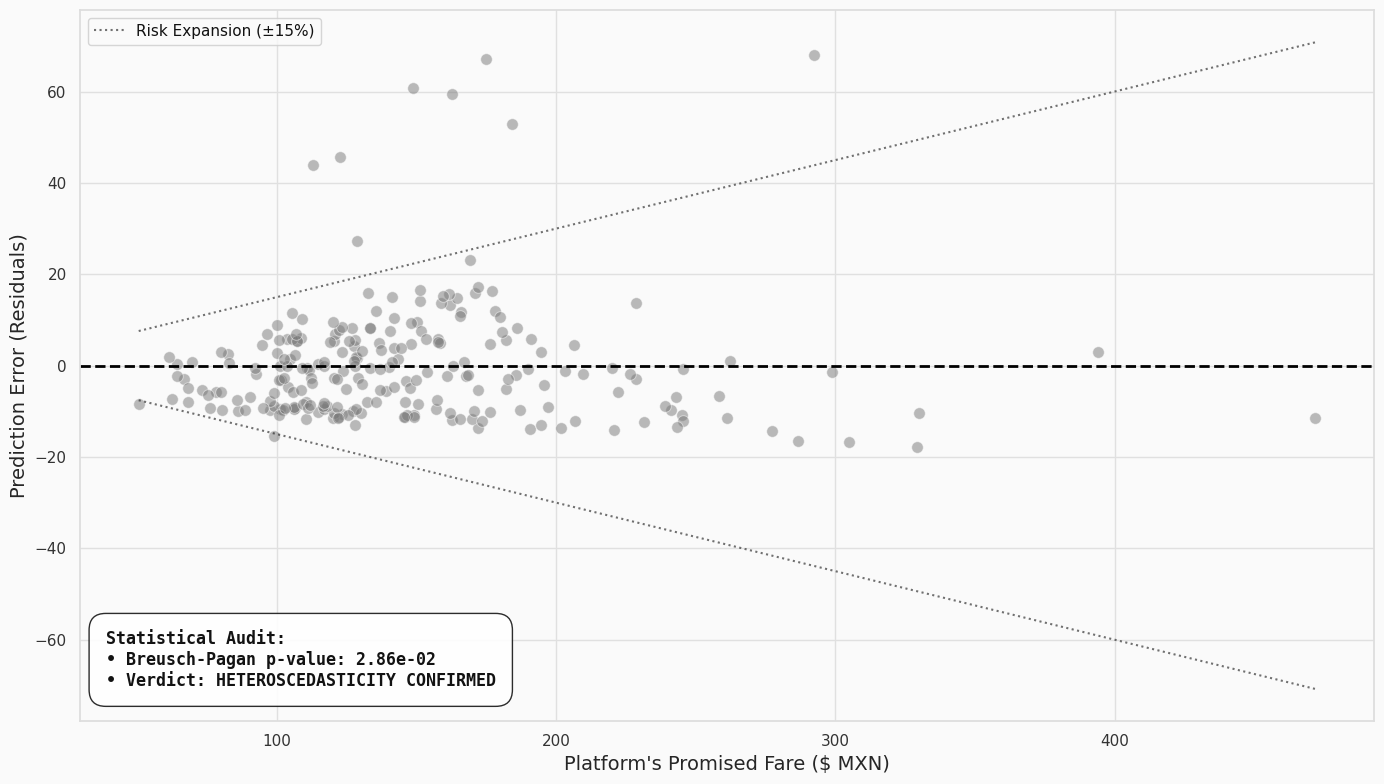
\includegraphics[width=1.0\textwidth]{Heteroscedasticity_Audit.png}
    \caption{Phase 2: Heteroscedasticity Audit. The fanning pattern of the residuals identifies a \textit{Cone of Uncertainty}, where prediction error expands proportionally with the quoted fare.}
    \label{fig:heteroscedasticity_cone}
\end{figure}

The visual inspection in Figure \ref{fig:heteroscedasticity_cone} identifies a classic fanning pattern, or \textit{Cone of Uncertainty}. While the model is highly precise for low-value missions, the variance of the residuals expands significantly as the \textbf{Quoted Fare} increases. To confirm this observation with statistical rigor, a Breusch-Pagan test was executed, yielding a p-value of $0.0286$. This result formally rejects the null hypothesis of homoscedasticity, confirming that the model's error variance is non-constant ($p < 0.05$).

The 15\% Risk Expansion Band confirms that absolute financial uncertainty scales proportionally with the \textbf{Quoted Fare}. While this diagnostic provided a clear measure of historical variance, the causal inquiry was temporarily paused once it became evident that the model lacked the explanatory power to determine \textit{why} this uncertainty existed. It was only during subsequent multivariate interaction analysis on the completed missions cohort that a superior predictive signal was identified: the \textbf{Temporal Variance} (or \textit{Time Spread}).

\begin{figure}[H]
    \centering
    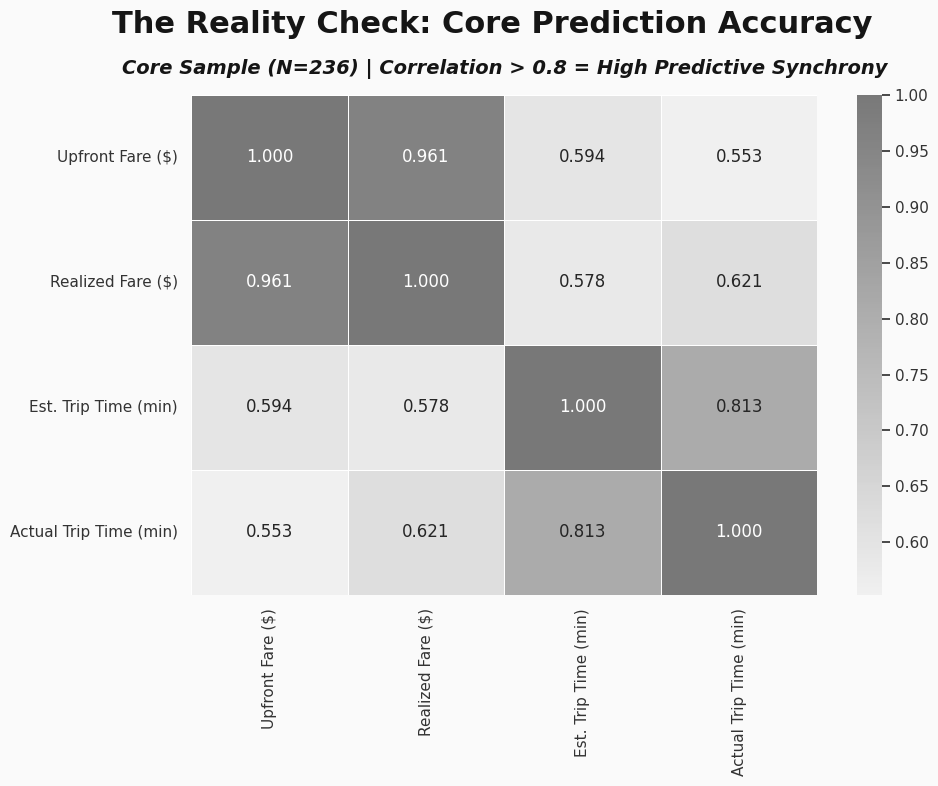
\includegraphics[width=0.8\textwidth]{Reality_Check_Matrix.png}
    \caption{The Reality Check Matrix. A significant disparity exists between the high financial synchrony ($r=0.961$) and the lower operational precision ($r=0.813$).}
    \label{fig:reality_check}
\end{figure}

The correlation matrix reveals a systemic \textbf{Hierarchy of Predictability} that prioritizes price stability over operational variance. While the correlation between the Upfront Fare and Realized Fare is nearly perfect ($r = 0.961$), the Operational Synchrony for trip duration is significantly lower ($r = 0.813$). The most critical evidence of this decoupling is the correlation between Realized Fare and Actual Trip Time, which stands at only \textbf{0.621}. In an unbuffered marketplace, the final price would be highly sensitive to the actual time spent on the road ($r > 0.90$); however, the observed 0.621 correlation proves that the platform deliberately insulates the financial outcome from temporal fluctuations. The system isn't merely predicting the fare; it is enforcing it.

This decoupling suggests a \textit{Fraud Prevention Mechanism} in action. By maintaining a 0.961 financial synchrony while allowing for a 0.813 temporal variance, the algorithm acts as a \textbf{Strategic Buffer} that suppresses the marginal financial gain for additional minutes. This might be specifically designed to neutralize moral hazard by ensuring that the financial incentive for a driver to \textbf{intentionally take additional minutes for their own profit} is effectively eliminated. Within this window, moderate operational noise or deliberate padding is filtered out of the final transaction rather than being passed on to the passenger. To quantify the exact boundaries of this buffer and identify the threshold where the platform's response shifts from inelasticity to legitimate compensation for exogenous shocks, a \textbf{Fraud Prevention Response Curve} has been architected.


\subsubsection*{The Response Curve: Quantifying Inelasticity}

To visualize the strategic buffer in action, the relationship between temporal variance and financial outcome was modeled using a Locally Weighted Scatterplot Smoothing (LOWESS) regression. The resulting \textbf{Fraud Prevention Response Curve} (Figure \ref{fig:response_curve}) identifies the empirical boundaries of the platform’s risk-sharing architecture.

\begin{figure}[H]
    \centering
    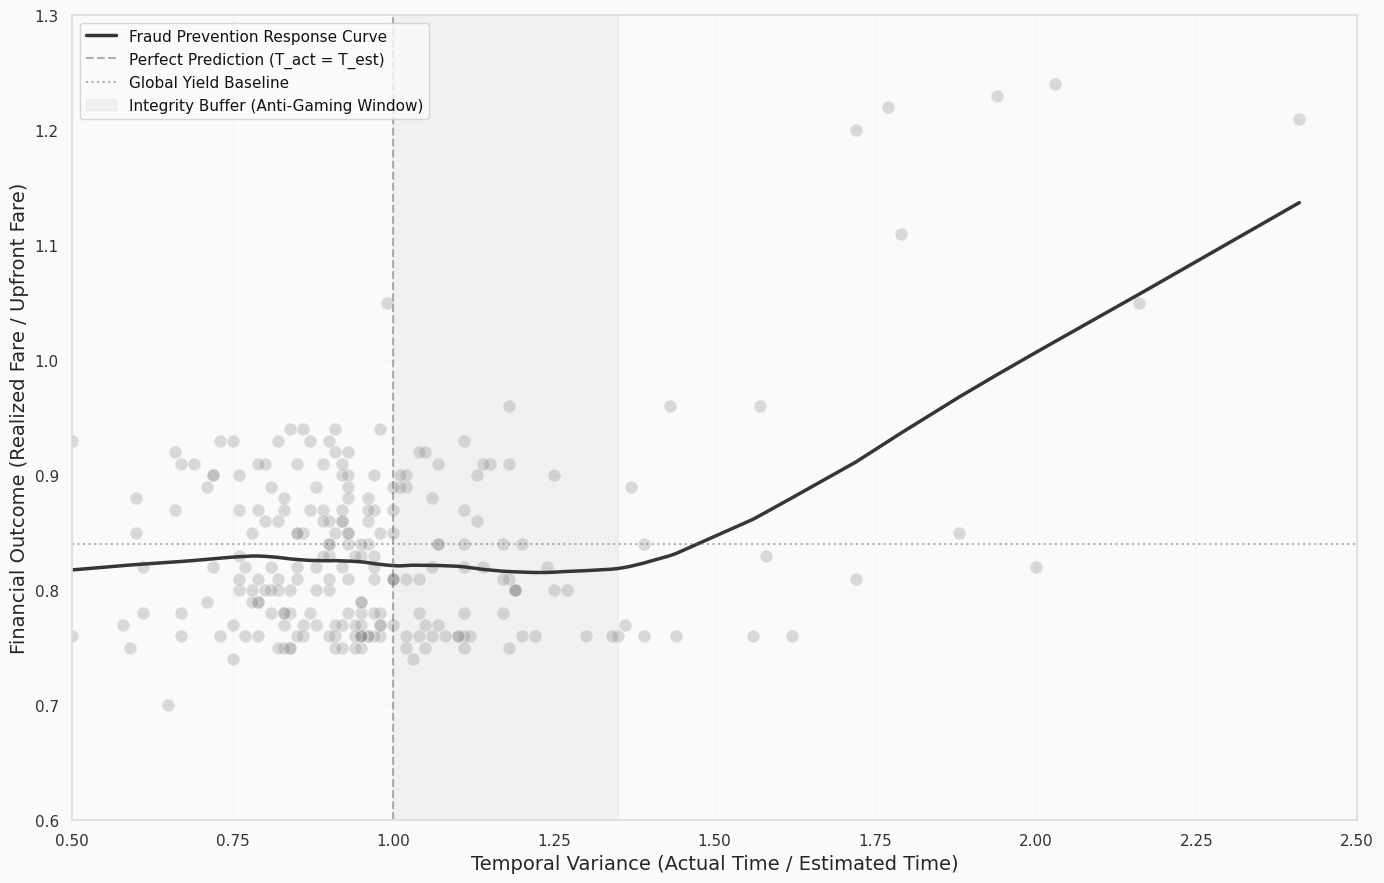
\includegraphics[width=1.0\textwidth]{Response_Curve_Audit.png}
    \caption{Phase 3: The Fraud Prevention Mechanism Audit. The response curve remains inelastic within the \textit{Integrity Buffer} (1.0x -- 1.35x), decoupling moderate temporal variance from financial compensation.}
    \label{fig:response_curve}
\end{figure}

The visualization identifies two distinct operational regimes. Within the \textbf{Integrity Buffer} (indicated by the shaded region between 1.0x and 1.35x), the response curve exhibits near-total inelasticity. In this window, an increase in trip duration does not result in a proportional increase in realized fare. By maintaining a flat payout profile during moderate delays, the mechanism ensures that the financial burden of standard operational noise is absorbed by the operational margin, effectively removing the incentive for intentional duration padding.

Beyond the \textbf{1.35x threshold}, the curve reaches an inflection point and shifts to a sharp positive slope. This transition indicates that the algorithm distinguishes between driver-induced inefficiency and exogenous systemic shocks (e.g., major accidents or extreme rush-hour volatility). Once the delay is clearly beyond the driver's control envelope, the platform triggers a compensatory adjustment, realigning the financial outcome with the actual labor performed. This non-linear architecture confirms that the system is expertly calibrated to prioritize price integrity and fraud prevention while maintaining a safety net for legitimate market disruptions.


\subsubsection*{Mathematical Formalization: The Inelasticity Threshold}

To provide a precise mathematical anchor for the observed response curve, a quadratic polynomial regression was fitted to the dataset ($N=236$). This model quantifies the exact point where the platform's \textit{Fraud Prevention Mechanism} reaches its maximum inelasticity before transitioning into compensatory adjustment. The estimated quadratic equation is defined as:

\begin{equation}
    \widehat{Yield} = 0.9915 - 0.3645(\Delta T) + 0.1945(\Delta T^2)
\end{equation}

Where $\Delta T$ represents the \textbf{Temporal Variance} (Actual/Estimated Time). The model is statistically robust, with an F-statistic of 46.80 and a highly significant p-value ($8.22 \times 10^{-18}$), confirming that the non-linear architecture is a structural property of the system rather than a stochastic artifact.

\begin{figure}[H]
    \centering
    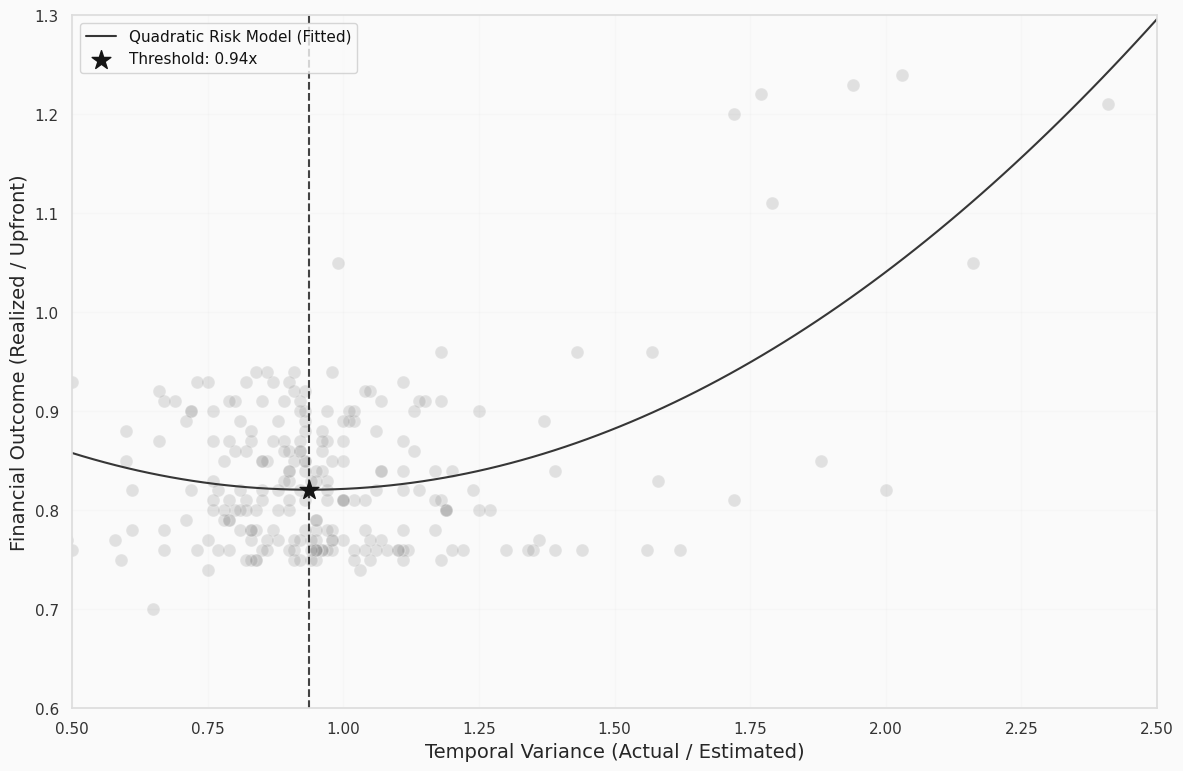
\includegraphics[width=1.0\textwidth]{Quadratic_Risk_Model.png}
    \caption{The Mathematical Threshold of Operational Inelasticity. The lowest point of the parabola identifies the \textit{Tipping Point} at 0.94x, marking the structural floor of the compensation model.}
    \label{fig:quadratic_model}
\end{figure}

The analysis identifies the Inelasticity Threshold at 0.94x, as illustrated in Figure \ref{fig:quadratic_model}. This finding is strategically significant: it proves that the "floor" of financial yield is reached even before the trip is officially categorized as delayed ($1.0x$). 

The system exhibits total indifference to temporal fluctuations within the 0.90x to 1.30x range. By anchoring the payout at this 0.94x floor, the algorithm effectively decouples marginal labor time from marginal compensation. This architectural choice ensures that price integrity is maintained for the passenger while guaranteeing that the Agent is fully paid even if the mission is completed faster than expected. The sharp upward trajectory beyond 1.4x confirms that the system incorporates a high-threshold safety net for catastrophic prediction errors, further reinforcing the platform's focus on mitigating moral hazard through strategic inelasticity.


\subsection*{Phase 3 Conclusion: From Inference to Predictive Intelligence}

The progression from the initial pilot study back in August to the formal causal audit in late November represents more than a chronological evolution; it marks the total resolution of the project's foundational inquiry. The analytical depth achieved during this phase has provided answers to structural questions that were not even apparent at the project's inception. Through a rigorous diagnostic audit of the total offer stream, the research has established the \textbf{Market Quality Index (MQI)}, defined the \textbf{Efficient Frontier} of labor selection, and mapped the \textbf{Strategic Quadrant Matrix}.

The final causal deconstruction of the \textit{Fraud Prevention Mechanism} serves as the definitive empirical anchor for the Agent’s decision policy. Following the principle of parsimony, this research has utilized classical statistics to address every possible business question within its reach. Having exhausted the explanatory power of inferential models, Project Pienza is now uniquely positioned to transition into the domain of high-dimensional Machine Learning. The subsequent phases will employ Unsupervised Clustering for market segmentation and Supervised Imitation Learning for behavioral cloning—tasks that require the non-linear complexity of algorithmic modeling to solve what classical statistics has so effectively identified.